\documentclass[12pt]{article}

% Packages
\usepackage{float}
\usepackage{amsmath}
\usepackage{amsfonts}
\usepackage{subcaption}
\usepackage{graphicx}
\usepackage{listingsutf8}
\usepackage[utf8]{inputenc}
\usepackage{xcolor}
\usepackage[a4paper, total={16cm, 23.7cm}]{geometry}
\usepackage[colorlinks=true,urlcolor=blue]{hyperref}
\usepackage{color}

% Compiler/IDE directives
% !TeX spellcheck = en_US

% General
\fontfamily{phv}
\captionsetup{width=0.8\textwidth}

% Graphicx
\graphicspath{ {images/} }
 
% Listings
\definecolor{codegreen}{rgb}{0,0.6,0}
\definecolor{codegray}{rgb}{0.5,0.5,0.5}
\definecolor{codepurple}{rgb}{0.58,0,0.82}
\definecolor{backcolour}{rgb}{0.95,0.95,0.92} 
\lstdefinestyle{mystyle}{
    backgroundcolor=\color{backcolour},   
    commentstyle=\color{codegreen},
    keywordstyle=\color{magenta},
    numberstyle=\tiny\color{codegray},
    stringstyle=\color{codepurple},
    basicstyle=\fontsize{7}{9}\selectfont\ttfamily,
    breakatwhitespace=false,         
    breaklines=true,                 
    captionpos=b,                    
    keepspaces=true,                 
    numbers=left,                    
    numbersep=5pt,                  
    showspaces=false,                
    showstringspaces=false,
    showtabs=false,                  
    tabsize=2
}
\lstset{style=mystyle}

% Geometry
\DeclareMathSizes{12}{13}{10}{8}
\setlength\parindent{0.7cm}

% Helper commands
\newcommand*\diff{\mathop{}\!\mathrm{d}}
\newcommand*\Diff[1]{\mathop{}\!\mathrm{d^#1}}
\newcommand\tab[1][.7cm]{\hspace*{#1}}
\renewcommand{\refname}{}
\newcommand{\code}[1]{\texttt{#1}}


%----------------------------------------------------------------------------
% THE DOCUMENT
%----------------------------------------------------------------------------
\begin{document}


%----------------------------------------------------------------------------
% TITLE
%----------------------------------------------------------------------------
\begin{center}
	\Huge Vectorization of the VELO-UT tracking\\
	\Large Short internal report\\
	\vspace{1pc}
	\huge Péter Kardos \\
\end{center}


Please check out the \textit{Design of the improved algorithm} section of \href{https://github.com/petiaccja/UU_CERN_Thesis/blob/master/Report/uu_cern_thesis_report.pdf}{my thesis report} for a detailed description of the algorithm itself. All code is on branch \href{https://gitlab.cern.ch/lhcb/Rec/tree/pkardos_PrVeloUtOpt}{pkardos\_PrVeloUtOpt}.


%----------------------------------------------------------------------------
% === ARTIFACTS ===
%----------------------------------------------------------------------------

\section{Artifacts}


\subsection{New VELO-UT algorithm \& hit handler}

\begin{itshape}
    Rec/Pr/PrVeloUT/src/\\
    \tab Constants.h\\
    \tab Constants.cpp\\
    \tab PrVeloUtOpt.h\\
    \tab PrVeloUtOpt.cpp\\
    \tab PrStoreUtHitOpt.h\\
    \tab PrStoreUtHitOpt.cpp\\
    \tab UtHitSpacePartition.h\\
    \tab UtHitSpacePartition.cpp\\
    \tab UtUtil.h\\
    \tab UtUtil.cpp
\end{itshape}

\vspace{1pc}

Next to the original \code{PrVeloUT} algorithm, I added another one called \code{PrVeloUtOpt}. The new algorithm, \code{PrVeloutOpt}, is mostly the same, but its code is in line with clean coding practices (as much as was possible) and it is vectorized and optimized. The \code{HitHandler} is replaced by the \code{UtHitSpacePartition} which uses uniform grid space partitioning instead of per-sector partitioning. The \code{PrStoreUtHitOpt} algorithm writes hits in this new scheme. \code{Contants} are hardcoded properties of the detector geometry, \code{UtUtil} contains solution to common problems such as accessing $B\ dL$ values.

\newpage
\subsection{SOA data model "framework"}

\begin{itshape}
    Rec/Pr/PrVeloUT/src/\\
    \tab SoaContainerify.hpp
\end{itshape}

\vspace{1pc}

Adds \code{resize}, \code{reserve} and \code{size} methods to SOA struct declarations using the boost::PFR library to discover and manipulate individual member variables at compile time.

Example:
\begin{lstlisting}[language=C++]
struct PointsBase {
    std::vector<float> x;
    std::vector<float> y;
    std::array<std::vector<int>, 3> meta;
};
using Points = SoaContainerify<PointsBase>;

Points points;
points.resize(10);
assert(points.x.size() == 10);
assert(points.y.size() == 10);
assert(points.meta[0].size() == 10);
assert(points.size() == 10);
\end{lstlisting}


\subsection{Supporting code}

\begin{itshape}
    Rec/Pr/PrVeloUT/src/\\
    \tab SimdUtil.h\\
    \tab StackAllocator.h\\
    \tab AlignedAllocator.hpp
\end{itshape}

\vspace{1pc}

\code{SimdUtil} contains some stuff to wrap Vc and give matching vector sizes for the VELO-UT algorithm. It also contains SIMD pruning helper function that are interoperable with Vc.

The \code{StackAllocator} is a simple STL allocator that acquires aligned chunks of memory from a large upfront memory pool.

The \code{AlignedAllocator} is an STL allocator that wraps STL'
s \code{aligned\_alloc} functions to force different alignment than 
\code{std::allocator\textless T\textgreater} would give. 
Disables zero-initialization of primitive arithmetic types such as \code{float}.


\subsection{Boost PFR library}

\begin{itshape}
    Rec/Pr/PrVeloUT/src/boost/*
\end{itshape}

\vspace{1pc}

A template metaprogramming helper library that provides a tuple-like interface for plain structs. Not officially part of boost.


\subsection{Auxiliary algorithms}

\begin{itshape}
    \tab Rec/Pr/PrMCTools/src/PrLHCbID2MCParticle.cpp
\end{itshape}

\vspace{1pc}

As the new algorithm no longer uses the \code{HitHandler}, the \code{PrLHCbID2MCParticle} had to be modified to extract the LHCbIDs from an \code{UtHitSpacePartition} object.


%----------------------------------------------------------------------------
% === IMPLEMENTATION ===
%----------------------------------------------------------------------------

\section{Implementation details}

\subsection{Overallocation}

Note that the code relies on underlying allocators allocating space with one more entire SIMD vector available at the end of the requested block. This is because the loops don't mask the last element, just read it regardless. The allocators giving the exact number of bytes allocated likely leads to segfaults and nasty things with SIMD loops. To fix this, masked reads and writes or at least documentation to the code could be added. The code is memory bound anyways, adding a mask calculation may not have any adverse effects on performance.


%----------------------------------------------------------------------------
% === RESULTS ===
%----------------------------------------------------------------------------

\section{Results}


In isolated benchmarks, on busy events, the optimized version is about 2.5 times faster than the original. In the framework, it is somewhat less. The old version produces 12300 evt/s whereas the new does 12600 with this and this configuration. \\
\textcolor{red}{TODO: add exact number and exact config}\\
\textcolor{red}{TODO: insert efficiency table from checker}


%----------------------------------------------------------------------------
% === INTEGRATION ===
%----------------------------------------------------------------------------

\newpage
\section{How to integrate, properly}

\subsection{Current state}

All it takes to get the new algorithm working is changing three lines in the configuration files to start using them. The algorithm runs properly and produces the expected results.


\subsection{Arranging files}

I added all new code to \textit{Rec/Pr/PrVeloUT/src/}, including support files and third party libs. That is obviously not correct. Boost PFR needs to be merged with boost in LCG. The helper files, such as the SOA framework and UT tools may be useful in other contexts, and should be moved accordingly.

\subsection{CMake dependencies}

\textit{Pr/PrMCTools/CMakeLists.txt} is forced to depend on a sibling library, \textit{Pr/PrVeloUT/CMakeLists.txt}, because it requires the definitions of the \code{UtHitSpacePartition}. This is not good, and it can be solved by moving \code{UtHitSpacePartition} (and all its dependencies) to LHCb, which is also not good because there is no other reason to move these files.

\textit{Pr/PrVeloUT/CMakeLists.txt} was hacked to emit a library to be consumed by \textit{Pr/PrMCTools/CMakeLists.txt}, which is not good either -- this is because MC matching (\code{PrLHCbID2MCParticle.cpp}) needs to definition of the \code{UtHitSpacePartition}. Additionally, it now depends on Vc libraries, that's perfectly fine. 


\subsection{Contants.h}

Most information in this file should be retrieved from geometry services instead of being hardcoded. The file should be deleted and the rest of the code updated accordingly.

\subsection{Namespaces, names}

Naming and namespaces are off, as there is not a clear convention in the current software. A clear convention should be decided and code adjusted to it.

\subsection{Compilation}

Flags AVX2, BMI and BMI2 need to be specified. This basically means Haswell.


%----------------------------------------------------------------------------
% === FUTURE WORK ===
%----------------------------------------------------------------------------

\newpage
\section{Future work and known issues}

\subsection{Align space partitioning properly on Y}

The uniform grid space partitioning should be tightly aligned to UT sensor rows. The grid's Y ticks should be exactly where the non-tilted sensors of the UT meet, possibly shifted a few millimeters up or down to make the most of the overlap of the UT sensors when the track hits at an angle. Currently I just took the upper and lower limits of the UT from the TDR an divided it into 14 equal rows.

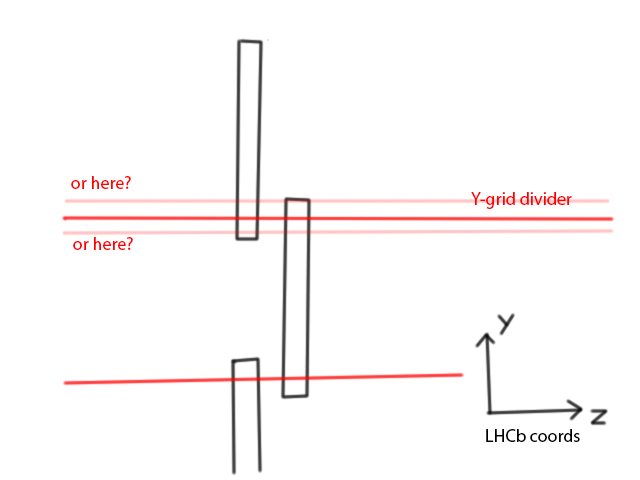
\includegraphics[width=0.9\textwidth]{images/y_grid_align.jpg}

\newpage
\subsection{Add double binning on Y}

Efficiencies are slightly lower compared to the original PrVeloUT, this is probably because there is no double binning on the Y axis - that is, only fiber hits from a single row are considered. In case the track hits between two rows, the overlap of the rows should take care of the problem, but for U and V layers hits may still be missed due to the tilt. By looking up both adjacent rows, one burns some more CPU cycles but it may help with efficiency. To be tried.

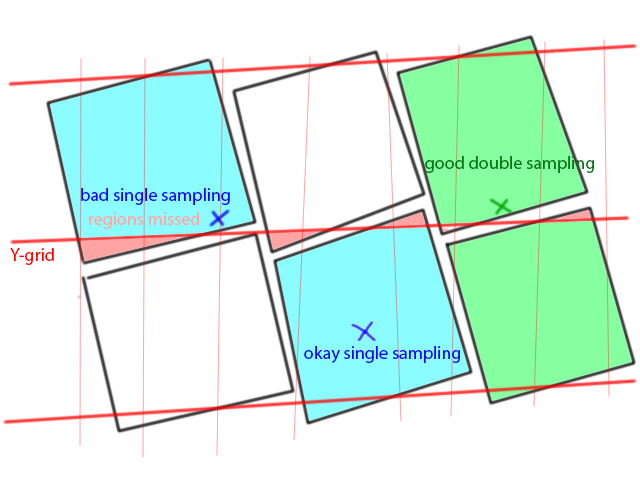
\includegraphics[width=0.9\textwidth]{images/y_double_binning.jpg}

\subsection{Vectorize aligned hit searching}

\code{FindLinesForTrack} is a heavy CPU consumer yet it is not vectorized at all. The loops are too small and branching makes it impractical. Maybe there is a clever way? Maybe a completely different algorithm? Maybe vectorizing it over tracks instead?


\subsection{AVX-512}

Should work without problems, where the algorithm needs the vector width it is acquired from a global constexpr \code{SimdWidth} which is currently acquired from Vc. The AVX2 emulation of the compressed store should be replaced with native intrinsics. Unfortunately, Vc does not support AVX-512, and the code is written with Vc.



\end{document}
